\documentclass[11pt,a4paper,titlepage,oneside]{report}

\usepackage[english]{babel}
\usepackage[utf8]{inputenc} % input encoding is UTF-8

\usepackage{graphicx}
\usepackage{tabularx}
\usepackage{subcaption}
\usepackage{apacite}
\usepackage{natbib}
\usepackage{color}
\usepackage[unicode,pdftex]{hyperref}
\usepackage{xcolor}

\hypersetup{
  colorlinks,
  linkcolor={red!50!black},
  citecolor={blue!50!black},
  urlcolor={blue!80!black}
}

\begin{document}

% Title page %%%%%%%%%%%%%%%%%%%%%%%%%%%%%%%%%%%%%%%%%%%%%%%%%%%%%%%%
\begin{titlepage}

\begin{figure}
\centering
\begin{subfigure}{.5\textwidth}
\centering

\includegraphics[width=0.8\textwidth]{img/logo_NTNU.png}\\
\end{subfigure}%
\begin{subfigure}{.5\textwidth}
\centering

\includegraphics[width=0.8\textwidth]{img/logo_SINTEF.jpg}
\end{subfigure}
\end{figure}

\begin{center}
{\LARGE \textbf{TDT4290 - Customer Driven Project}}
\vfill
{\Huge \textbf{Ocean forecast}}

\vspace{12pt}
{\LARGE \textbf{SINTEF}}

\vspace{30pt}
{\LARGE \textbf{Final report}}
\vfill
{\LARGE \textbf{Autumn 2014}}
\end{center}
\vfill
\begin{tabular*}{\textwidth}{@{\extracolsep{\fill}} l l}
\textbf{Group 6} & \textbf{Advisor} \\
Arve Nygård & Gleb Sizov \\
Anders Smedegaard Pedersen & \\
Emil Jakobus Schroeder & \\
Hans Kristian Henriksen & \\
Marco Radavelli & \\
Ondřej Hujňák & \\
Ruben Håskjold Fagerli & \\
\end{tabular*}

\end{titlepage}

% Empty page %%%%%%%%%%%%%%%%%%%%%%%%%%%%%%%%%%%%%%%%%%%%%%%%%%%%%%%%
\newpage
\thispagestyle{empty}
\mbox{}
\newpage

% Abstract %%%%%%%%%%%%%%%%%%%%%%%%%%%%%%%%%%%%%%%%%%%%%%%%%%%%%%%%%%
\begin{abstract}
Abstract
\end{abstract}

% Signatures %%%%%%%%%%%%%%%%%%%%%%%%%%%%%%%%%%%%%%%%%%%%%%%%%%%%%%%%
\thispagestyle{empty}
\begin{center}
{\large \textbf{Trondheim, \today}}\\
\vspace{2.5cm}
\begin{tabularx}{\textwidth}{@{\extracolsep{1cm}} X X }
\dotfill & \dotfill \\
~Arve Nygård & ~Anders Smedegaard Pedersen \\[1cm]
\dotfill & \dotfill \\
~Emil Jakobus Schroeder & ~Hans Kristian Henriksen \\[1cm]
\dotfill & \dotfill \\
~Marco Radavelli & ~Ondřej Hujňák \\[1cm]
\dotfill & \\
~Ruben Håskjold Fagerli & \\[1cm]
\end{tabularx}
\end{center}

% Table of contents %%%%%%%%%%%%%%%%%%%%%%%%%%%%%%%%%%%%%%%%%%%%%%%%%
\tableofcontents
\addtocontents{toc}{\protect\thispagestyle{empty}}

% List of figures %%%%%%%%%%%%%%%%%%%%%%%%%%%%%%%%%%%%%%%%%%%%%%%%%%%
\listoffigures
\addtocontents{lof}{\protect\thispagestyle{empty}}

% List of tables %%%%%%%%%%%%%%%%%%%%%%%%%%%%%%%%%%%%%%%%%%%%%%%%%%%%
\listoftables
\addtocontents{lot}{\protect\thispagestyle{empty}}

\pagenumbering{arabic}
\setcounter{page}{0}

% Main body %%%%%%%%%%%%%%%%%%%%%%%%%%%%%%%%%%%%%%%%%%%%%%%%%%%%%%%%%
%%%%%%%%%%%%%%%%%%%%%%%%%%%%%%%%%%%%%%%%%%%%%%%%%%%%%%%%%%%%%%%%%%%%%

\chapter{Introduction}
\section{TDT 4290 - Customer driven project}
The task is set forth in the subject TDT 4290 - Customer driven project at the Norwegian university of science and technology. The goal of the course is 
\begin{quote}
(...)to give the students a practical experience of carrying out all the phases of a typical customer guided IS/IT-project. \citep{TDT4290:Intro}
\end{quote}
The subject divides the students into random groups, and assigns each group an assignment. The assignments are real problems that businesses needs solved. 

Although the assignment is to follow the entire process of an IT-project, the focus is on the earlier phases of a project. Thus, an important part of the assignment is the work leading up to the implementation phase. There is obviously also an important focus on the implementation itself. Maintenance is however left out of the scope of the projects.

\section{Customer}
The customer is SINTEF Fisheries and Aquaculture (SINTEF Fiskeri og havbruk AS). 
SINTEF was founded in 1950 and it is nowadays organized into 8 divisions. The division of Fisheries and Aquaculture was founded in 1999 and represents technological expertise and industry knowledge in the utilization of renewable marine resources. Under the vision \"Technology for a better society\" it works for a knowledge-based bio marine industry. Its goal is to meet market demands for technological research and development on renewable marine resources.

\section{Ocean currents}
About currents, why they are important, who is interested etc.

\section{Assignment and scope}
The client, SINTEF Fisheries and Aquaculture, has given us the project labeled ”Ocean Forecast”. The task is to improve the actual system of storing and retrieving data for the monitored and predicted parameters of ocean.

\chapter{Planning}
This section will give an overview of our plans for the project. It will include time estimation, group organization, risk management and quality assurance.

The name of the project and the scope of the assignment has already been introduced in the previous section.
\section{Project stakeholders}
The stakeholders of this project are the following:
\begin{description}
\item[Project owner (customer)] SINTEF Fisheries and Aquaculture
\item[Supervisor (from NTNU)] Gleb Sizov
\item[Examiner] External examiner, nominated by the direction of the course TDT4290 - Customer Driven Project
\item[Team members (students)] 
\end{description}

\section{Background for the project: software system development}
The customer owns a working solution, running on its own servers, for the delivery and analysis of marine tracked and predicted data, in form of maps with overlays and charts.
The background for this project is to optimize the actual, slow and memory-consuming solution, with a new one, and/or creating new front-end application using those data, to cover more use-cases.

\section{Measurement of project effects}
Some predefined criterias must be met in order to consider out project a successful one. Our product must be working according to the requirements and pass all tests in order to be a success. All requirements prioritized high and medium must be fulfilled. Requirements that have low priority are optional, but should be implemented if there is sufficient time.
In our case, quite open goals were requested by the customer, and no precisely quantifiable measurements were defined.
If working on improving the actual solution the measurements should be:
\begin{itemize}
\item The time it takes to visualize data for the end user should be “reasonably low” even with slow internet connection (like from Chile) or from a mobile device
\item The same displayed features as the actual working system are still available
\end{itemize}
If working on new use cases, the measurements should be:
\begin{itemize}
\item The same displayed features as the actual working system are still available
\item New features (such as mobile app and new charts) are added in order to cover more use-cases 
\end{itemize}
In both cases, an open source based solution is considered to be better than a commercial one.

\section{General terms}
The choice implementation language, platform and tools to use are up to us. The requirement is that the solution should run on a server.
There are non-functional requirements, in terms of improving performance and storage consumption, that should be accomplished.

\section{Planned workload}
Group members will aim to work 24-25h on average per week, for a total amount of 12 weeks. Group members can distribute the workload among days according to their lecture timetibles, as long as deadlines (including sprints deadlines) are met.
Our group consists of 7 people, so that the weekly average amount of workload is globally around 168-175h, for a total of 2016-2100 h.

\section{Schedule of results}
We are using a Scrum-like project management framework, and working prototypes are expected to be produced at the end of each speint. Requirements have been prioritized by the customer with numbers from 1 to 100. The requirements for our project are inevitably overlapping, and almost all the requirements must be accomplished in order to produced a working solution, to satisfy the basic project goal requested by the customer.

\section{Concrete project work plan}
This section describes the specific layout of the project. This project follows the Scrum methodology with some variants introduced, as discussed in the appendix. The first five weeks were spent planning, pre-studies (which included a preliminary implementation of the critical part of the system), and writing the requirement specification. As a common practice, the project was divided into sprints. We decided to make each sprint lasting one week. At the end of the last sprint all the requirements should be accomplished.
\subsection{Phases}
We decide to the Scrum methodology, so that Scrum sprints characterize the phases of the project.
The following are the phases that can be distinguished in the project:
\begin{itemize}
\item Initiation phase (pre-planning)
\item Project Planning
\item Project Prestudy Sprint (Sprint 0)

\item Sprint 1
\item Pre-delivery of report (17th October)

\item Sprint 2
\item Sprint 3
\item Sprint 4

\item Demo Planning
\item Project Delivery and Demonstration
\end{itemize}

\subsection{Activities}
\begin{description}
\item[Pre-planning] During the pre-planning activity, the group members know each other and understand the task. There are also the first meetings with the customer and with the avisor.
\item[Pre-study and planning] The pre-study and planning activity is the stage where the actual work on the project begins. We explpore solutions and we determine which technologies will be used and how the product will be realized.
\item[Documentation] The documentation activity represents time spent documenting the work effort, including implementation, research etc., and administrative tasks like status reports and documents for the meetings.
\item[Coordination] The coordination activity is accomplished throughout the project, and consists of activities to coordinate the work, such as meetings, internal emails, calls and messages.
\item[Implementation] The implementation activity consists of the implementation of the system. This includes the programming of both the back end and the front end part.
\item[Testing] The testing activity represents time spent testing the system. This includes integration testing, unit testing, functional testing and scenario-driven testing.
\item[Presentation] The presentation activity is the final presentation of the system and the delivery of the report.
\end{description}

\subsection{Milestones}
We defined some milestones in order not to create delays in the progress of the project.
There are some milestones defined by the course structure, and we decided to add some more "internal" project milestones in order to avoid delays.
The following are the defined milestones:
\begin{description}
\item[October 6th] Pre-study phase to be completed
\item[October 17th] Pre-delivery of report (defined by the course coordinators)
\item[November 17th] Project report to be completed
\item[November 20th] Final presentation day (defined by the course coordinators)
\end{description}

\subsection{Person-hours per activity and phase + lectures + project management}
In this projects there have been a number of guest lectures, and we have made sure that every lecture were attended by at least one member in the team.

\section{Project Organization}
\subsection{Organizational diagram of how the group is organized}

\begin{figure}[h]
\begin{center}
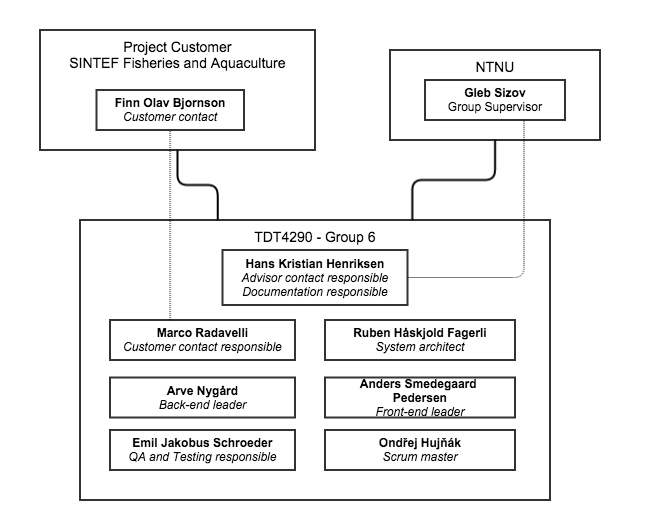
\includegraphics[height=260px,width=328px]{img/tdt4290_group_6_organizational_structure.png}
\caption{Organizational diagram. The arrows indicate the bi-directional communication. The dotted arrows denotes the preferred way of communication between components. Note that the layout is not hierarchical and it is arranged this way only to better fit on the printed page.}
\label{fig:organizational-structure}
\end{center}
\end{figure}

\subsection{Roles and corresponding responsibilities}
We defined and diveded roles and responsibilities among group members. We agreed the distribution of the responsibilities by the voluntary choice of the role for each component of the group, and internal unanimous agreement.
We conveyed the following roles:
\begin{description}
\item[Scrum master] His task is to make sure that we meet our goals, he is the first person who talks to the customer and to the advisor in the meetings, make sure that the groups meetings have a structure and that they finish on time. According to the scrum methodology, the scrum master also has to supervide the scrum pocess (control that is respected), remove eventual impediments to the team's work, protect team from distracting influences, and make sure that the team is on-task.
\emph{Role assigned to: \textbf{Ondřej Hujňák}}
\item[Customer contact] His task is to arrange customer meeting, forward customer emails to the group if needed, and ensure that all the needed communication with the customer is done.
\emph{Role assigned to: \textbf{Marco Radavelli}}
\item[QA and testing responsible] Ensure that the implementation fulfills the requirements, design test plan, define and ensure that the Quality Assurance standard is followed during the project.
\emph{Role assigned to: \textbf{Emil Jakobus Schroeder}}
\item[Documentation responsible] Supervise the structure and the content of all the documents (report, status reports, agenda and minutes of meetings, pre-study report). Main responsible to take notes during meetings. 
\emph{Role assigned to: \textbf{Hans Kristian Henriksen}}
\item[Advisor contact] Arrange advisor meetings, send documents (status report, agenda and minutes of last meeting) to the advisor before each meeting.
\emph{Role assigned to: \textbf{Hans Kristian Henriksen}}
\item[Front-end leader] Supervise the front-end architecture and implementation, and coordinate the front-end developer team
\emph{Role assigned to: \textbf{Anders Smedegaard Pedersen}}
\item[Back-end leader] Supervises the back-end architecture and implementation, and coordinate the back-end developer team
\emph{Role assigned to: \textbf{Arve Nygård}}
\item[System architect] Make sure that there is consistency between requirements, design and implementation, and that the design is feasible and reasonable.
\emph{Role assigned to: \textbf{Ruben Håskjold Fagerli}}
\end{description}

\subsection{Weekly schedule}
We decided to adopt a scrum-like model of software development, with internal group meetings twice a week, weekly meetings with the advisor and meeting with the customer when needed (typically every other week). The schedule is defined as follows:
\begin{itemize}
\item Mondays 2-3 pm - Advisor meeting
\item Mondays 3-4pm - Team meeting
\item Thursdays 12-2pm - Team meeting
\end{itemize}
For weeks 37 and 38 the advisor meeting will be Thursday 4pm.

We decided to use the academic quarter for internal meetings, but to start the meeting at the time conveyed sharp for advisor meetings.

\chapter{Tools and technology}
\section{Documents}

  \subsection{\LaTeX}
  \LaTeX~is a typesetting system and document markup language that became standard for scientific documents. It is easily expandable by thousands of different packages and can handle all aspects of scientific papers.

  We have chosen to use \LaTeX~for our report for two main reasons - \LaTeX~sources are easily readible and, because they are simple text files, they can be easily versioned by various version control systems. Second reason was focus on content, not on form. In \LaTeX~sources there is only very little information about exact view of the page. \LaTeX~itself during compile time chooses the best position of elements so it complies with all typographic norms.

  We have created a template in our shared space together with a bibliography file. Everyone could then write his sections in an environment that suited him the best while the current state of the report was always available to all members.

  \subsection{Google Docs}
  Google Docs \footnote{\url{https://docs.google.com}} is a web based office suite including a text editor, a spreadsheet program and a presentation program. All files created in these programs can easily be shared with colaborators. By sharing files the colaborators get access to view and edit the files. Editing and commenting on other's work. We decided to use Google Docs for all documents that did not require the advanced typesetting of \LaTeX~so we had a common platform for such documents.

\section{Project management}
  \subsection{Trello}
Trello is a web-based collaborative project management tool originally made by Fog Creek Software (New York, USA) \footnote{\url{http://www.fogcreek.com/}}. 
It's based on the Kanban method which has first implemented by Toyotain 1953 to be used in car production. It has since been modified to be used in several different industries. 
David J. Anderson formulated a model based on Kanban for knowlegde based work, specifically software development, where the team work incrementally pulling work from a queue \citep{da2004}. 
This work queue in represented by a card for each task wich is located in a "to-do" area on a board. Task may then be moved to a bin called for example "in progress" to indicate that the task is beeing work on. Finally, when the task is complete, the cars can be moved to a "done" bin. In Trello this is implemented by elements you can drag and drop between bins. As an administrator you have the possibility to define both bins and boards which makes Trello a very versatile tool.  
Trello is a freemium webservice which means that it is free to use but additional support and features can be accessed if you pay a fee. As we only needed the standard functions and thus used the free version.
  \subsection{Slack}
Slack is a webbased team communication tool founded by Stewart Butterfield. It offers text chat in different channels and integration with a number of different popular services used by development teams \footnote{\url{https://slack.com/integrations}}. This was useful to us since we needed to share information that might be more relevant to specific team members and also to have a single means of communication. Using Slack's integration with Trello and Github we would get notified when there where changes on these platforms aswell. Slack's posibillity to share files, or link to files on Google Documents also came in handy.

\section{Version control}
  \subsection{Git}
  Git is a distributed version control system developed in 2005 by Linus Torvalds and Linux development community \citep{ProGit}. Git was made to be small, fast and easy to use especially for code management as it's main purpose was versioning of Linux kernel source code. Nowdays is Git one of the most used versioning controls systems in software development thanks to it's open linence and powerfull features.

  We have chosen Git because some members already know it and are able to work efficiently with it. Another advantage is easy branching and distributed architecture that allows you to work offline. 
  
  We have created an organization on GitHub\footnote{\url{https://github.com}} with multiple repositories for different separate parts of our work - reports, server sources, client sources. We have chosen GitHub because it is well known git hosting server that offers advanced features and stability. Moreover some members already had accounts on GitHub and were familiar with interface, which shortened time needed to setup a working environment.

\section{Programming languages}
  \subsection{Java}
  Java is a popular programming language developed by a team led by James Gosling at Sun Microsystems in 1991. It's full-featured , general purpose language capable of developing robust mission-critical applications \citep{liang}. This and the fact that everybody in the group had at least basic knowlegde of Java led to the dessicion that we would use Java for our back-end application.  
  \subsection{JavaScript}
  As stated by Davis Flanagan i JavaScript: the definitive guide "Javascript is part of the triad of technologies that all Web developers must learn". He continues to note that JavaScript specifies the behaviour of the web page \citep{fd11}. Along with specification of HTML5 and ECMAscript 6 (the standard name of JavaScript) the posibilities of what you can achieve with JavaScript has greatly improved. Since our assignment was to create a web based solution it seamed natural to use JavaScript as part of the solution. This was further supported by the excistence of open source libraries designed to make interactive maps which was relevant for our assginment.

\section{IDEs}

\chapter{Pre study}
In this chapter, we present the findings of the pre study. The pre study document was made as a separate document that was meant to be delivered to the customer independently of this report. Therefore, there are overlapping sections with the full report. These sections will not be given in this chapter, but are instead presented in their respective chapters of the full report. 

\chapter{Requirements}

\chapter {Pre-sprint work}

\chapter{Sprint 1}

\chapter{Sprint 2}

\chapter{Sprint 3}

\chapter{Sprint 4}

\chapter{Final solution}

\chapter{Evaluation}


% Sources cited in the document
% uncomment when there are some citations, uncomment bibtex in Makefile
%\bibliographystyle{plain}
\bibliographystyle{apacite}
\chapter{Bibliography}
\begin{flushleft}
	\bibliography{report}
\end{flushleft}

% Appendixes
\appendix

\end{document}
